\documentclass{article}
% Packages
\usepackage{titlesec}
\usepackage{indentfirst}
\usepackage{amsmath, amsthm, amssymb, graphicx}
\usepackage{graphicx}
\usepackage[pages=-]{background}
\usepackage{xcolor}
\usepackage{caption}
\usepackage{booktabs}

\backgroundsetup{
  scale=1,
  angle=0,
  opacity=1,
  color=black,
  position=current page.north east,
  vshift=-1.5cm,
  hshift=-2.5cm,
  contents={
    
\includegraphics[width=2cm]{../source/Universitaet_Logo_RGB.pdf}
  }
}
% Title
\title{Satellite Lab1}
\author{Group6: Zhengyang Hua, Xipeng Li, Yushuo Feng}
\date{\today}


\begin{document}

\maketitle

\section{Introduction}


\section{Orignal Data}
\subsection{ITRF2008 IGS station}
The ITRF is The International Reference Frame,  
and ITRF2008 is a realization of the International Terrestrial Reference System 
that uses as input data time series of station positions and EOPs provided by the Technique Centers of the four space geodetic techniques (GPS, VLBI, SLR, DORIS).

In the file "ITRF2008\_GNSS.SSC.txt", we can find the coordinates of different stations at epoch 2005.0.
 and Time is given as the yyyy.yyyy format, which is the number of decimal years:
\begin{figure}[htbp]
    \centering
    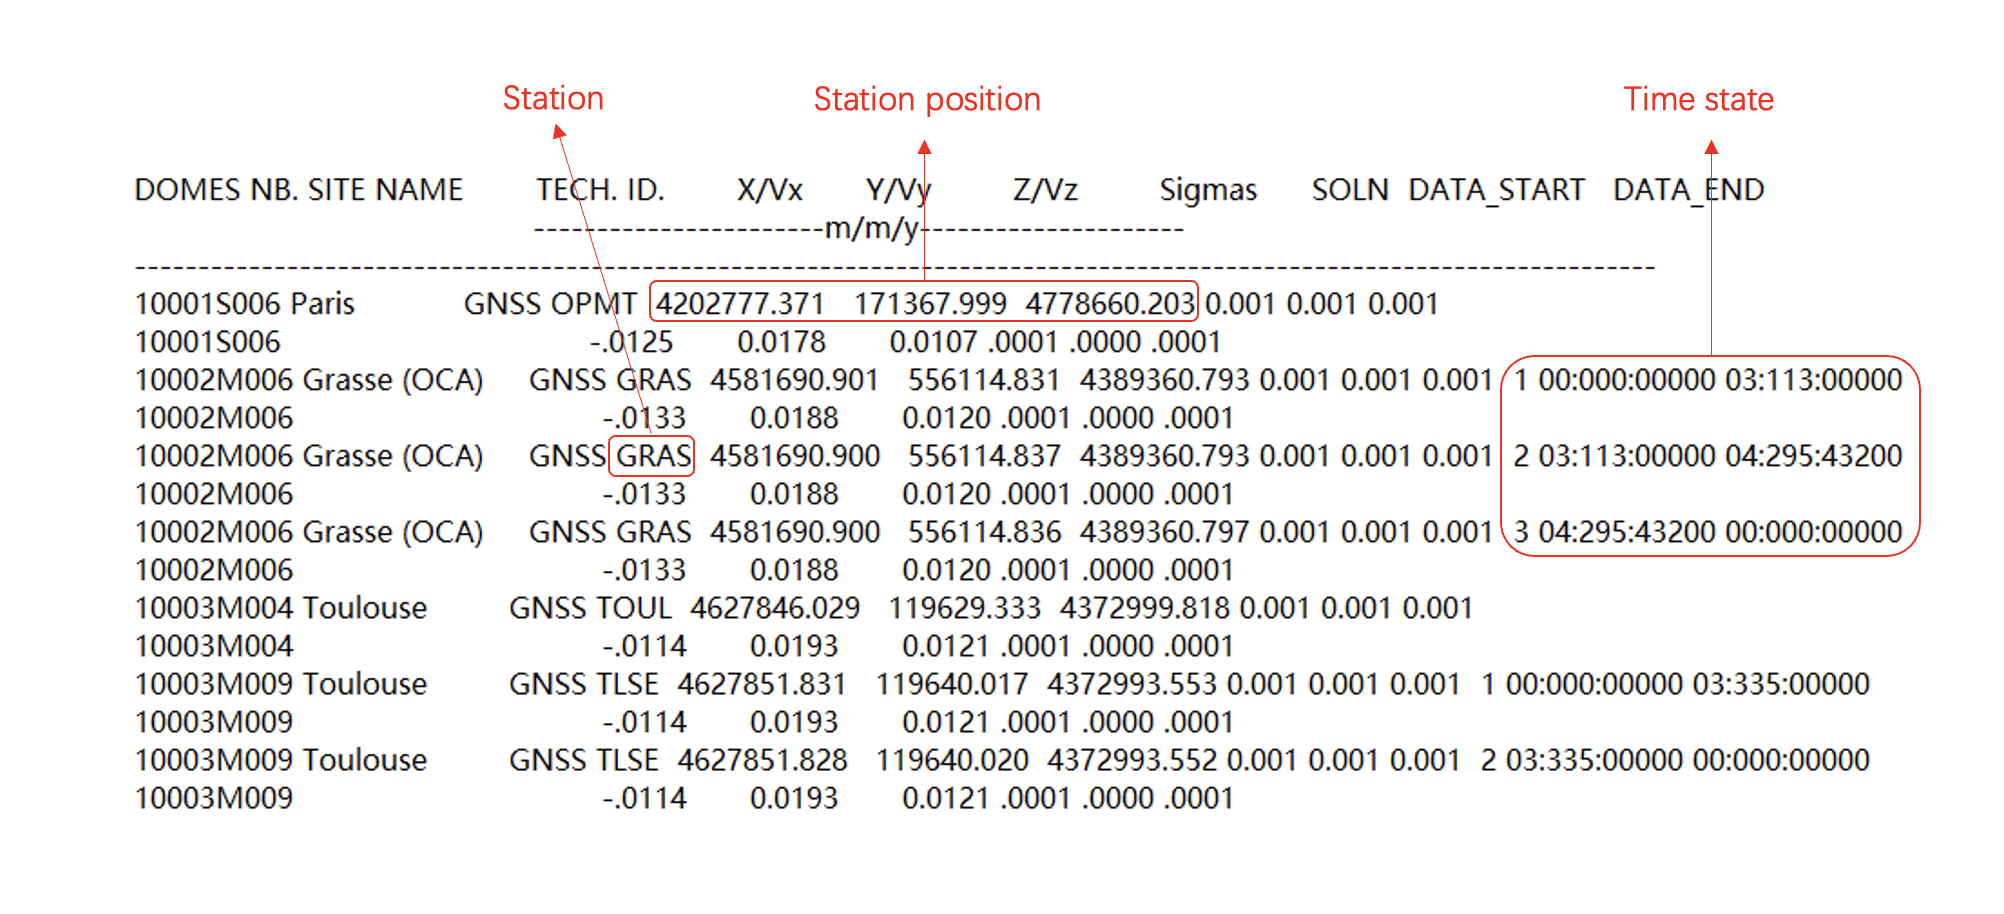
\includegraphics[width=12cm]{./source/ITRF2008.png}
    \caption{ITRF2008\_GNSS.ssc.txt Description}
    \label{fig:ITRF2008}
\end{figure}
\subsection{Station GPS Obversations}
We were responsible for the computation of the positions and movements of three measurement stations: KIRU, MORP, and REYK. The locations are illustrated in the following figure:

An example of the observation file for each data set is provided below, including two time formats and XYZ coordinates.
\begin{figure}[htbp]
    \centering
    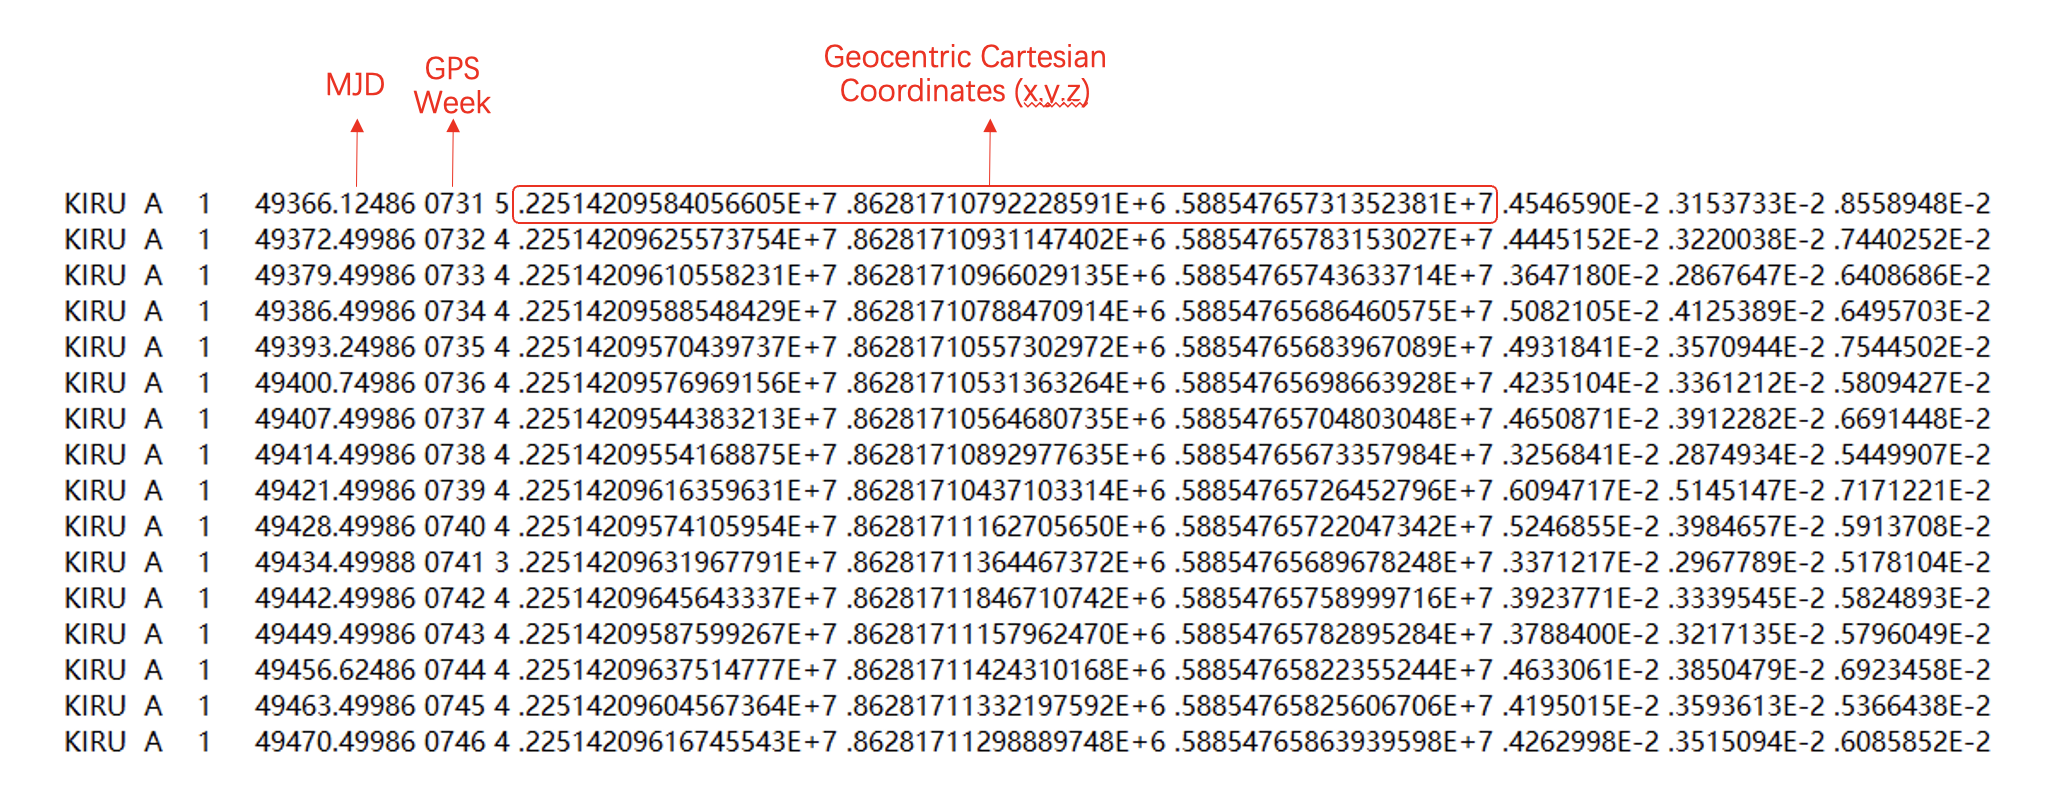
\includegraphics[width=12cm]{./source/xyz.png}
    \caption{station.xyz Description}
    \label{fig:XYZ_obs}
\end{figure}

And the file Discontinuities\_snx provides the discontinuity information in the positions' time series. The reasons for that include change of antenna and receiver, earthquake and so on.
In this example(station: REYK), the discontinuity happened three times due to earthquake, antenna change and unknown reason.
\begin{figure}[htbp]
  \centering
  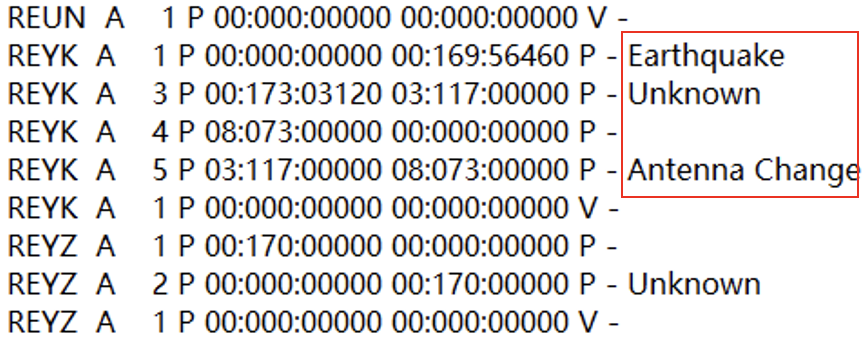
\includegraphics[width=12cm]{../source/dis.png}
  \caption{Discontinuities in time series}
  \label{fig:Dis_snx}
\end{figure}

\subsection{NUVEL 1A Model}
NUVEL(Northeast University Velocity) is a the collective term for geophysical Earth models that describes observable
continental movements through a dynamic theory of plaet tectonics.

The "NNR\_NUVEL1A.txt" gives the rotation referred to epoch $t_0$. 
The file contains the following data, where the leftmost column represents the station name, 
and in that row, the angular velocity changes in three directions are provided (unit: radians per million years or $rad/My$).
\begin{figure}[htbp]
    \centering
    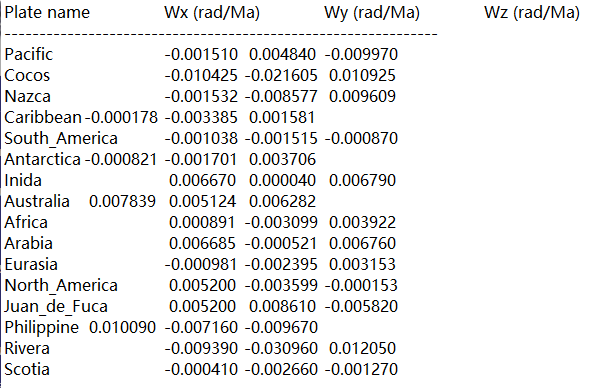
\includegraphics[width=12cm]{../source/nuvel.png}
    \caption{NUVEL\_1A.txt Description}
    \label{fig:Nuvel-1A}
\end{figure}
\subsection{GIA Models}

\subsection{Other data}

\subsection{Matlab Code}

\section{Methodology}
\subsection{Transoformation to LHS}
[Geocentric cartesian coordinate system] is a three-dimensional, earth-centered reference system in which locations are identified by their x, y, and z values. 
The x-axis is in the equatorial plane and intersects the prime meridian (usually Greenwich). 
The y-axis is also in the equatorial plane; it lies at right angles to the x-axis and intersects the 90-degree meridian. 
The z-axis coincides with the polar axis and is positive toward the north pole. The origin is located at the center of the sphere or spheroid.

[Local horizontal system] uses the Cartesian coordinates(East,Nort,Up) to represent position relative to a local origin. The local origin is described by the geodetic coordinates.

The initial coordinates are in the geocentric Cartesian coordinate system and need to be transformed into representation in the local horizontal coordinate system.
In this project, we use two angles and the ITRF2008 point positions as the original point, 
\begin{figure}[htbp]
  \centering
  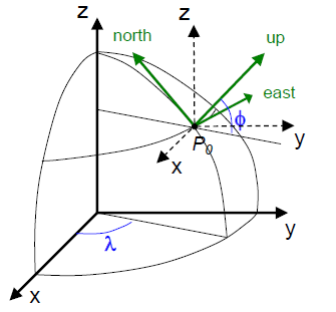
\includegraphics[width=6cm]{../source/transform.png}
  \caption{Coordinates Transformation}
  \label{fig:2lhs}
\end{figure}

Calculate the angle according to stations' geodetic coordinates:

$$\lambda=\arctan\frac{y}{x}$$ 
$$\varphi=\arctan\frac{2}{\sqrt{x^{2}+y^{2}}}$$

Then we can get the rotation matrix:
$$R_2(\delta)=\begin{pmatrix}\cos\delta&0&-\sin\delta\\0&1&0\\\sin\delta&0&\cos\delta\end{pmatrix}\quad R_3(\delta)= \begin{pmatrix}\cos\delta&\sin\delta&0\\-\sin\delta&\cos\delta&0\\0&0&1\end{pmatrix}$$

Transformation of coordinates:
$$\left.\begin{pmatrix}x_{up}\\x_{east}\\x_{north}\end{pmatrix}=R_2(-\varphi^0)R_3(\lambda^0)\left(\begin{pmatrix}x_1\\x_2\\x_3\end{pmatrix}\right.-\begin{pmatrix}x_1^0\\x_2^0\\x_3^0\end{pmatrix}\right)$$
$x^0$are the stations' geodetic coordinates, and $x$ is observations in file '.xyz'.
Notice that we also can directly use the longitude and latitude of stations provided in the file "Discontinuities\_CONFIRMED.snx".

In terms of velocity, its transformation into LHS only requires multiplication by a rotation matrix.
\subsection{Least Square Adjustment for Parameters Estimation}
For time series, $$ y(t)=\beta_{1}+\beta_{2}t+\beta_{3}\mathrm{cos}\omega t+\beta_{4}\mathrm{sin}\omega t $$
among which $\beta_3$ and $\beta_4$ are total amplitude of annual, and $\beta_2$ is linear trend; so we can build model like:
$$\begin{pmatrix}y(t_1)\\\vdots\\y(t_n)\end{pmatrix}=\begin{pmatrix}1&t_1&\cos\omega t_1&\sin\omega t_1\\\vdots&\vdots&\vdots&\vdots\\1&t_n&\cos\omega t_n&\sin\omega t_n\end{pmatrix}\begin{pmatrix}\beta_1\\\beta_2\\\beta_3\\\beta_4\end{pmatrix}$$
We can simppfit the model like: $$Y=X\beta+\varepsilon$$
where $Y$ is the observations, $X$ is the design matrix, $\beta$ is the parameters, and $\varepsilon$ is the noise.

According to least square, minimize the noise, 
derivative the square of noise and set it to zero so we get:
$$\beta=(X^TX)^{-1}X^TY$$ through this we can get the estimated parameters.

\subsection{Model of Plate Tectonics}
The movement of any plate on a spherical Earth can be described through a rotation around the Euler pole:
$$\underline{\Omega}=(\Omega_{1},\Omega_{2},\Omega_{3})^{T}$$
In point $\underline{x}_{0}=(x,y,z)^{T}$ the velocity vector v is obtained by:
$$\underline{v}=\underline{\Omega}\times\underline{x}_0=\begin{pmatrix}0&&-\Omega_z&&\Omega_y\\\Omega_z&&0&&-\Omega_x\\-\Omega_y&&\Omega_x&&0\end{pmatrix}\begin{pmatrix}x\\y\\z\end{pmatrix}$$

\subsection{Program Description}

\section{Results and Analysis}
\subsection{Time Series and Linear Trend}
Through the least square adjustment, out group get the time series of these three stations as shown below:
And we can see that the linear trend of KIRU in Up, East and North directions are , , and respectively.
\begin{figure}[htbp]
  \centering
  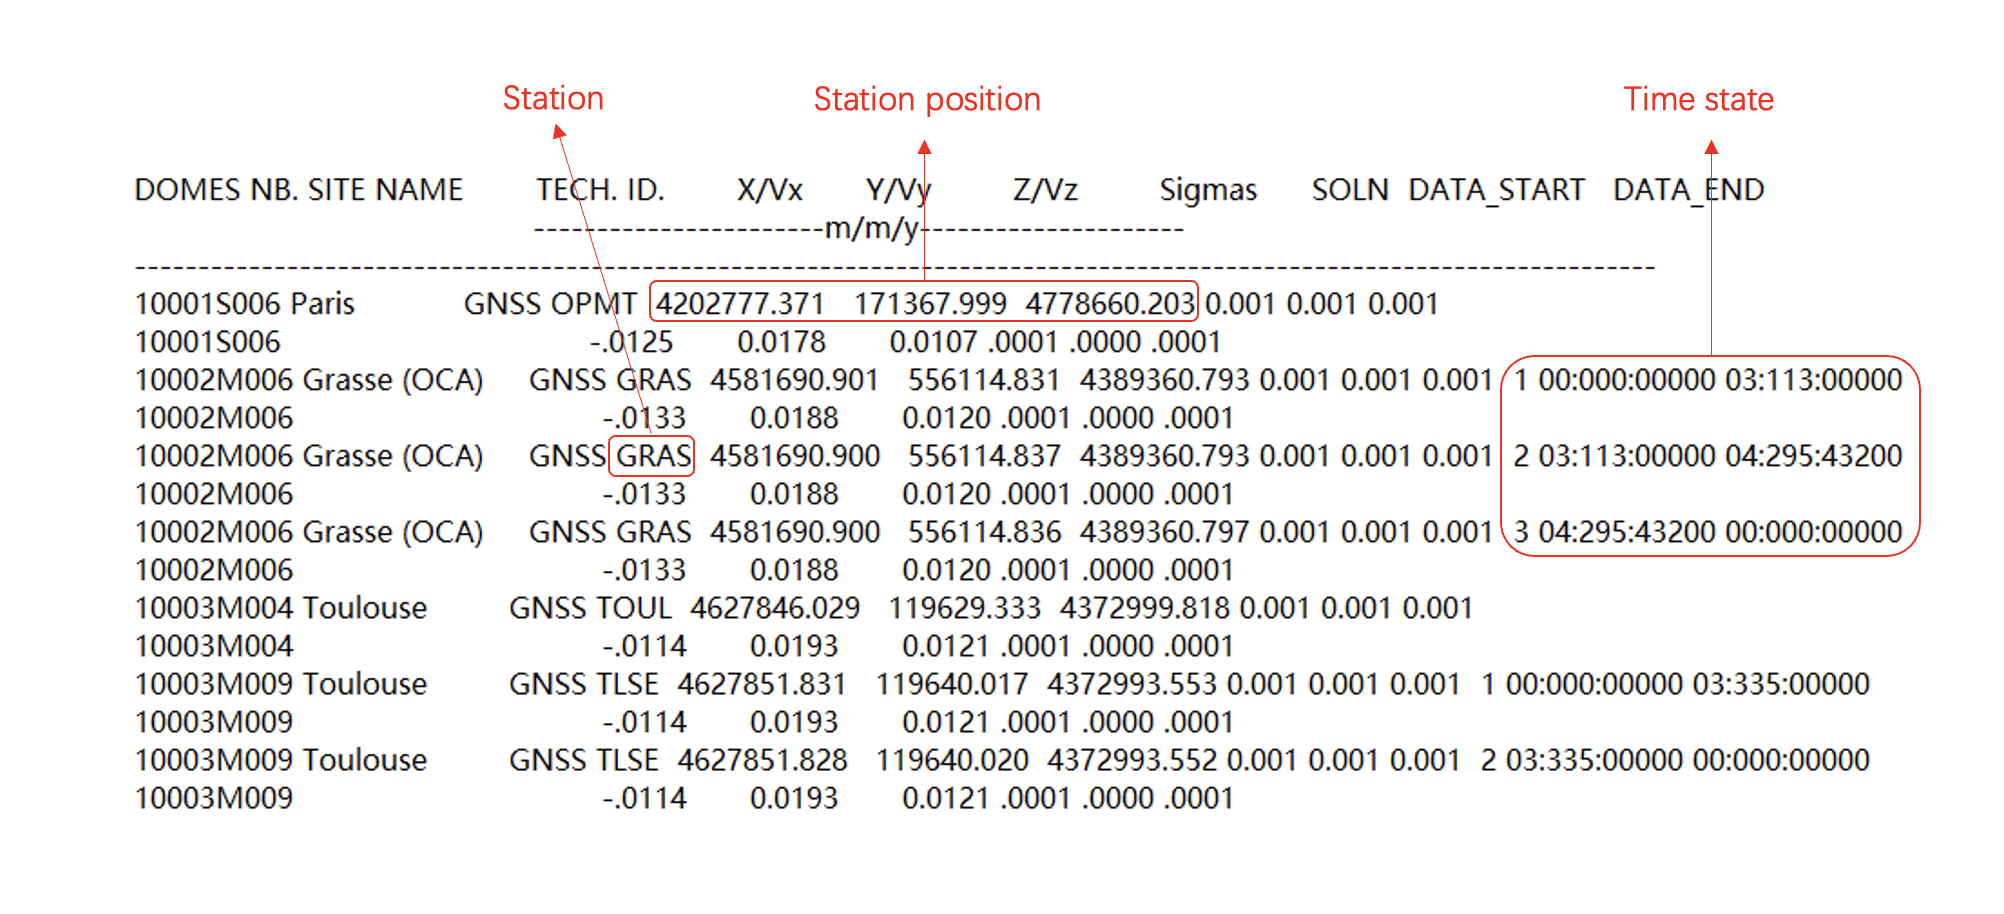
\includegraphics[width=10cm]{./source/ITRF2008.png}
  \captionsetup{skip=0.2cm}
  \caption{Time Series of KIRU}
  \label{fig:Ori_KIRU}
\end{figure}
\begin{figure}[htbp]
  \centering
  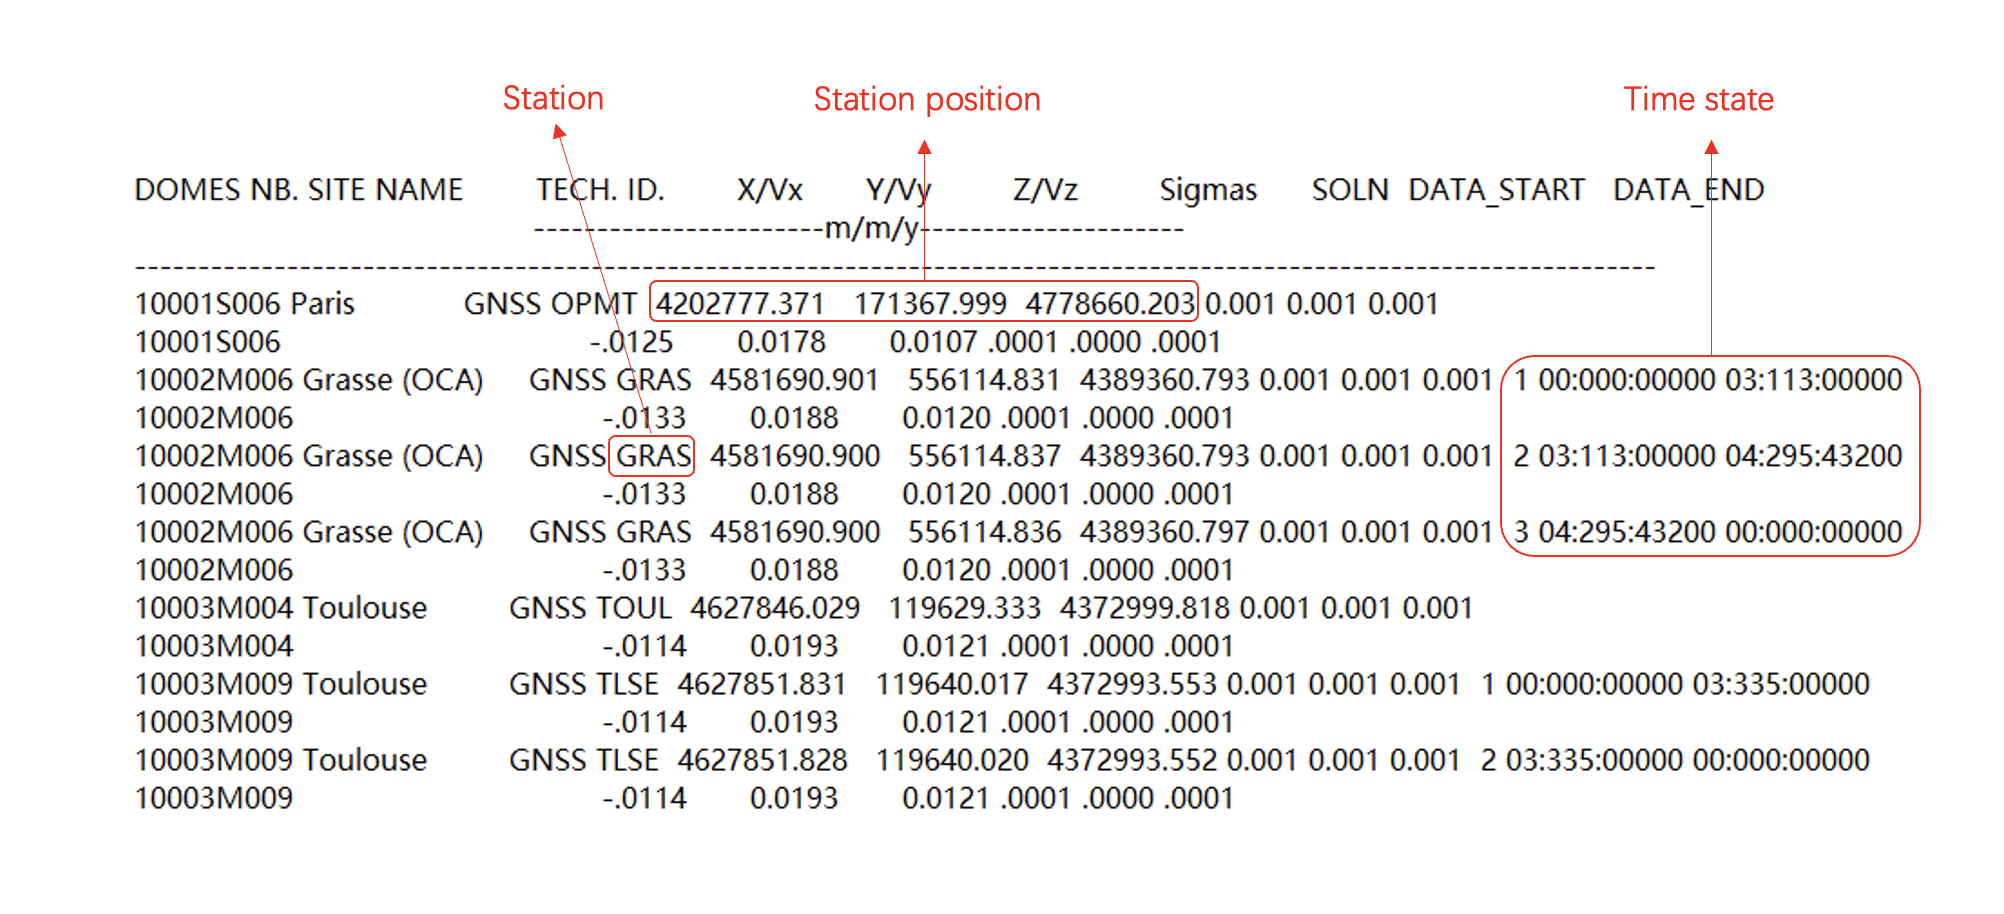
\includegraphics[width=10cm]{./source/ITRF2008.png}
  \caption{Time Series of MORP}
  \label{fig:Ori_MORP}
\end{figure}
\begin{figure}[htbp]
  \centering
  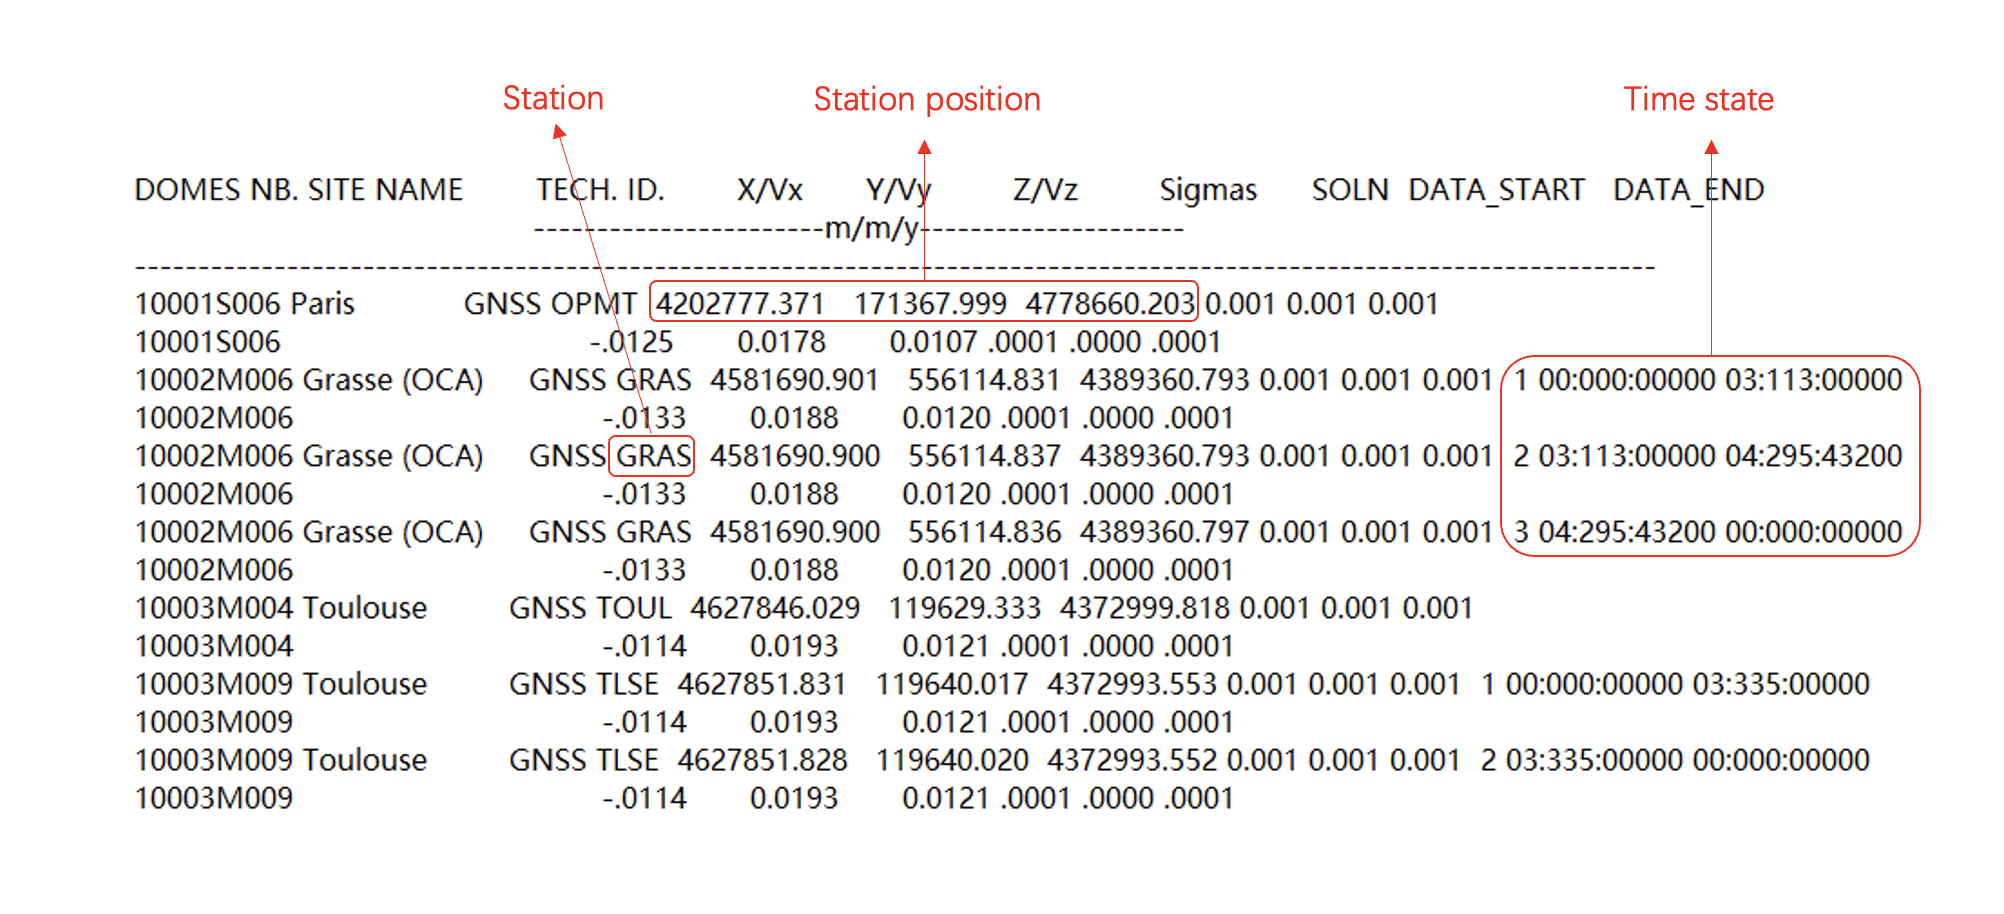
\includegraphics[width=10cm]{./source/ITRF2008.png}
  \caption{Time Series of REYK}
  \label{fig:Ori_REYK}
\end{figure}

\begin{table}[htbp]
  \centering
  \caption{Linear Trend of Time Series}
    \begin{tabular}{lrrr}
    \large Station & \multicolumn{3}{c}{\large Linear Trend(mm/y)} \\
    \midrule
          & \multicolumn{1}{l}{\large UP} & \multicolumn{1}{l}{\large EAST} & \multicolumn{1}{l}{\large NORTH} \\
          
     KIRU  &       &       &  \\[3pt]
     MORP  &       &       &  \\[3pt]
     REYK  &       &       &  \\
    \end{tabular}%
  \label{Tab:lin_trend}%
\end{table}%


\subsection{Comparison of horizontal movements}

\subsection{Comparison of vertical movements}

\section{Conclusion}

\end{document}
